\begin{summary}
\section{Contexte}
Ce laboratoire a servi d'introduction à la programmation temps réel sur
système embarqué (ici STM32).
Le XF (execution framework) a été développer pour être multiplateforme.
Une première version en C++ sur PC a été développer (avec la librairie Qt) pour 
déboguer au mieux tous les problèmes, ce qui aurait été complexe sur un système
embarqué.\\
Des tests communs aux deux systèmes (embarqués et PC) sont fournis, ainsi qu'une
structure de base du projet.
\end{summary}

\section{XF}
Le XF (execution framework) est un framework servant à piloter plusieurs machines
d'états finies en pseudo-parallèle.
\begin{figure}[H]
    \centering
        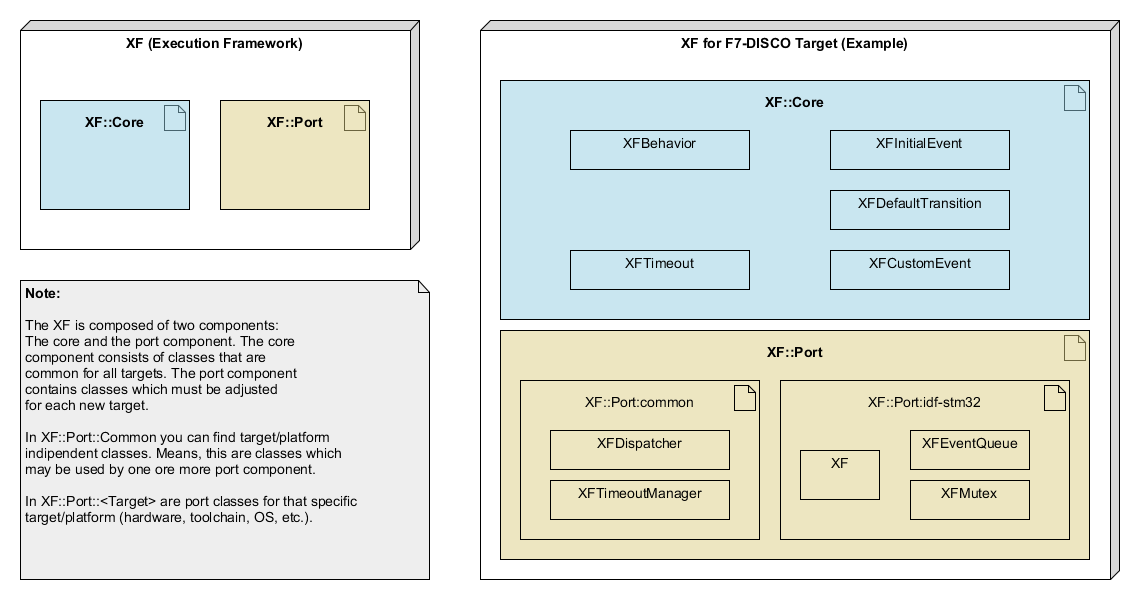
\includegraphics[width=\textwidth]{Images/xf/comp-simple-xf.png}
        \caption[Diagramme de composant de classe du XF]{Diagramme de composant de classe du XF 
        (provenant de la documentation \emph{Simplified XF}\footnotemark)}
\end{figure}

\footnotetext{\cite{documentation}}